\chapter{The Distributed Contact Discrete Element Method}

The Distributed Contact Discrete Element Method (DCDEM) \cite{canelas} is a variation of the Discrete Element Method wherein the \textbf{Contact Forces }$F^T_i$  acting on the $i^{th}$ particle due to collision with the $j^{th}$ particle is decomposed into \textbf{Normal} and \textbf{Tangential components}, $F_n$ and $F_t$, respectively. Both $F_n$ and $F_t$ are further resolved as \textbf{Repulsive} and \textbf{Dissipative} forces, $F^r$ and $F^d$, coming into existence due to the deformation of the material and the dissipation of energy during the deformation respectively. The DEM mechanisms in two interacting particles is as shown in Figure \ref{fig:dem_mechanism}.

\begin{figure}[htb!]
 \begin{subfigure}{.5\textwidth}
  \centering
    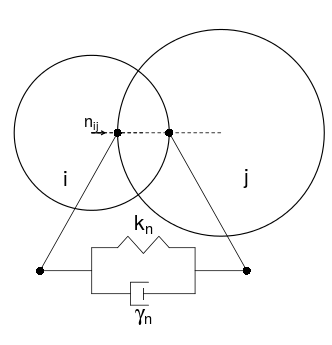
\includegraphics[width=\linewidth]{figures/normal_interaction.png} 
    \caption{{\small{Normal Interation}}}
 \end{subfigure}
 \begin{subfigure}{.5\textwidth}
  \centering
    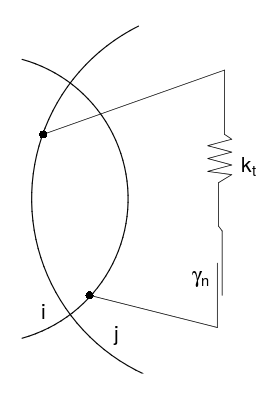
\includegraphics[width=.69\linewidth]{figures/tangential_interaction.png}
    \caption{{\small{Tangential Interaction}}}
     \end{subfigure}
 \caption{Scheme of DEM Mechanism (reproduced from \cite{canelas})}
 \label{fig:dem_mechanism}
\end{figure}
\newpage
The Normal Contact forces are given by a modified, non-linear Hertzian model as:

\begin{eqnarray}
{\bf{F}} = {\bf{F}}_n^r + {\bf{F}}_n^d = k_{n,ij}~\delta _{ij}^{3/2}~{\bf{e_{ij}}} - \gamma _{n,ij} ~ \delta _{ij}^{1/4} \dot{\delta _{ij}}~\bf{e_{ij}}  
\end{eqnarray}

{\raggedright{where,}}\\
$k_{n,ij} = $ Normal Stiffness Constant of the pair \textit{ij}\\
$\gamma _{n,ij} = $ Normal Damping Constant\\
$\delta _{ij} = $ Particle Overlap $= max(0, \frac{(d_i + d_j)}{2} - {\bf{|{\it{r_{ij}}}|}})$, $d_i, d_j = $ Particle diameter\\
${\bf{e_{ij}}} = $ Unit vector between two mass centers\\
$\dot{\delta _{ij}} = $ Rate of Normal Deformation $= \vec{\it{v_{ij}}}\cdot {\bf{e_{ij}}}$\\

The Stiffness and Damping constants are expressed in terms of the Young's Modulus $E$, Poisson's Ratio $\nu$ and the masses of the $i^{th}$ and $j^{th}$ as:

\begin{eqnarray}
 k_{n,ij} = \frac{4}{3} E^* \sqrt{R^*} \hspace{0.375cm} ; \hspace{0.375cm} \gamma _{n,ij} = C_n \sqrt{6M^*E^* \sqrt{R^*}}
\end{eqnarray}

{\raggedright{where,}}\\
$\frac{1}{E^*} = \frac{1-\nu_I^2}{E_I}+\frac{1-\nu_I^2}{E_I}$ \hspace{0.375cm} ; \hspace{0.375cm} $R^* = \frac{r_i r_j}{r_i + r_j}$ \hspace{0.375cm} ; \hspace{0.375cm} $M^* = \frac{m_I m_J}{m_i + m_j}$\\
with $C_n$ of the order of $10^{-5}$\\
E$_I$, E$_J =$ Young's Modulus of the I$^{th}$ and J$^{th}$ bodies\\
$\nu_I$, $\nu_J =$ Poisson's Ratio of the I$^{th}$ and J$^{th}$ bodies\\
r$_i$, r$_j =\sqrt{x^2+y^2+z^2}$, where $x,y,z$ are the co-ordinates of the i$^{th}$ and j$^{th}$ particles\\

The Tangential Contact Forces are given by a Linear Hertzian model bounded by a modified Coulomb Friction Law; the Coulomb Friction Law is modified by means of a sigmoidal function to account for the discontinuity coming into existence when the tangential velocity of the interacting bodies is zero \cite{vetsch}. The model is given as:

\begin{eqnarray}
 {\bf{F}}_{t,ij} = min(\mu_{f,IJ} {\bf{F}}_{n,ij}\tanh(8\dot{\delta^t_{ij}}){\bf{e^t_{ij}}}~; {\bf{F}}_t^r + {\bf{F}}_t^d)
\end{eqnarray}

\hspace{3.15cm}with,

\begin{eqnarray}
 {\bf{F}}_t^r + {\bf{F}}_t^d = k_{t,ij}~\delta^t_{ij}~{\bf{e^t_{ij}}} - \gamma _{t,ij} ~ \dot{\delta ^t_{ij}}~\bf{e^t_{ij}}
\end{eqnarray}

{\raggedright{where,}}\\
$\mu_{f,IJ} = $Coefficient of Kinetic Friction between interacting bodies I and J\\
$\delta^t_{ij} = $ Particle Overlap for Tangential interaction \\
${\bf{e^t_{ij}}} = $ Unit Vector of tangential component of relative velocity perpendicular to $F_n$\cite{vetsch}\\
$k_{t,ij} = $ Tangential Stiffness Constant $= \frac{2}{7} k_{n,ij}$ \cite{hooman}\\
$\gamma_{t,ij} = $ Tangential Damping Constant $=\frac{2}{7} \gamma_{n,ij}$\cite{canelas_thesis}\\
$\dot{\delta ^t_{ij}} = $ Rate of Tangential deformation \\

Since this work makes use of the particle approximation of the SPH method, particle overlap during both normal and tangential interaction is assumed to be given by the same form; $\dot{\delta ^t_{ij}}$, however, was extrapolated from that of $\dot{\delta _{ij}}$. Thus, the values of the  $\delta^t_{ij}$ and $\dot{\delta ^t_{ij}}$ were taken to be equal to $\delta_{ij}$ and $ \vec{\it{v^t_{ij}}}\cdot {\bf{e_{ij}}}$ respectively. 

Based on the definition, 
\begin{eqnarray}
 {\bf{e^t_{ij}}}            &=& \vec{v_{ij}} - \frac{(\vec{v_{ij}} \cdot \vec{F_{n,ij}}) \vec{F_{n,ij}}}{(|\vec{F_{n,ij}}|^2)} \nonumber\\
                            &=& \vec{v_{ij}} - \left(\vec{v_{ij}}\cdot\frac{\vec{F_{n,ij}}}{|\vec{F_{n,ij}}|}\right)\frac{\vec{F_{n,ij}}}{|\vec{F_{n,ij}}|} \nonumber\\
                            &=& \vec{v_{ij}} - \left(\vec{v_{ij}}\cdot{\bf{e_{ij}}}\right){\bf{e_{ij}}}\nonumber\\
 \therefore {\bf{e^t_{ij}}} &=& \vec{v_{ij}} - \dot{\delta_{ij}}{\bf{e_{ij}}}\nonumber
\end{eqnarray}


\section{PySPH Implementation}

\subsection{Data Structures and Software Constructs}
As mentioned in Section \ref{sec:pysph_abstractions}, the particle containers can be given additional properties based on the specific requirements of the problem. These are supplied as a ``constants'' dictionary with the keys as the property names and the values as a numpy array. This mechanism is used to provide physical properties such as Young's Modulus, Poisson's Ratio and Coefficient of Kinetic Friction. Further, since the model requires to calculate ${\bf{e_{ij}}}$, the center of masses of all the entities at the initial state of the system are also provided as constants\footnote[11]{The \lstinline!RigidBodyMoments()! class takes care of the evolution of the system mass centers thereafter}. Additionally, in order to demarcate individual solid bodies, the ``body\_id'' constant array is used. 

The interaction between bodies is divided as ``sources'' and ``destinations'', with the ``sources'' contributing to the overall disturbing force on the system and the  ``destinations'' being subjected to those forces. For implementing the new model, the destinations are additionally equipped with five constant arrays: Fx, Fy, Fz, check\_bit, and Fmag. The roles that these arrays play is listed in Table \ref{tab:dest_array}.

\begin{table}[htb!]
\centering
\begin{tabular}{|c|L|}
    \hline
    \textbf{Array Name} & \textbf{Role}\\
             &\\\hline
    Fx       & Array elements hold X Component of Total Collision Force of the destination bodies \\\hline
    Fx       & Array elements hold Y Component of Total Collision Force of the destination bodies \\\hline
    Fx       & Array elements hold Z Component of Total Collision Force of the destination bodies \\\hline
    check\_bit & Binary values of the array elements indicate if the destination body has been considered for force calculation\\\hline
    Fmag     & Magnitude of Maximum Collision Force acting on the destination body \\\hline
\end{tabular}
\caption{\small{Role of Additional Constant Arrays}}
\label{tab:dest_array}
\end{table}

Also, as introduced in section \ref{sec:pysph_abstractions} PySPH has Miscellaneous routines to allow ease in setting up cases and implementing models. These include the \lstinline!loop()! and \lstinline!post_loop()! methods described below:

\begin{itemize}

\item \lstinline!loop()!: This method loops over all the destination array particles ``one by one'' (along with the associated nearest neighbours) in each stage of the integrator step thereby allowing all the necessary force computations on each particle to be performed individually. 

\item \lstinline!post_loop()!: This method loops over all the destination array particles ``at once'' in each stage of the integrator step thereby allowing manipulations to all the particles after the individual computations are all completed.
\end{itemize}

The \lstinline!loop()! and \lstinline!post_loop()! methods can take specific arguments as dictated by the physics of the problem. These arguments could be pre-fixed with ``\textbf{s\_}'' and ``\textbf{d\_}'' to associate with the source or destination particle properties. Further, general SPH computations make use of many terms which are common across various domains and are provided as ``Pre-computed Symbols''\footnote[12]{\url{http://pysph.readthedocs.io/en/latest/design/overview.html\#writing-the-equations}} to facilitate easy reuse; these terms also feature as arguments in the \lstinline!loop()! and \lstinline!post_loop()! methods.

Lastly, as mentioned in Section \ref{sec:pysph_design}, PySPH incorporates Run Time Code Generation (RTCG) to generate C/C++ extensions for all simulations. Therefore, while implementing the model any data structures necessary must be declared such it is parsed and understood by the Cython Code Generator. This can be done by making use of the \lstinline!declare()! function. By default, all explicitly undeclared variables are considered as doubles.

\subsection{Flowchart of DCDEM Implementation}

The flowchart of the implementation is as shown below. Appendix \ref{appendix2} shows the PySPH implementation of the algorithm. 
$\vspace{0.5cm}$

 \tikzstyle{decision} = [diamond, draw, text width=4.5em, text badly centered, node distance=3cm, inner sep=0pt]
 \tikzstyle{block1} = [rectangle, draw, text width=10em, text centered, rounded corners, minimum height=4em]
 \tikzstyle{block2} = [rectangle, draw, text width=15em, text centered, rounded corners, minimum height=4em]
 \tikzstyle{line} = [draw, -latex',]
 \tikzstyle{cloud} = [draw, ellipse, minimum height=2em]
 \tikzstyle{circle} = [draw, ellipse, minimum height=1em] 
 \tikzstyle{mytext} = [text width=0.5cm,text centered]

\begin{table} [!htb]
 \begin{tabular}{ccc}
  \begin{tikzpicture}[node distance = 2cm]
    \node [cloud] (start) {start};
    \node [block1, below of=start] (init) {Call Constructor of Parent Class and Initialize C$_n$};
    \node [block1, below of=init,node distance=2.5cm] (loop) {Call \lstinline!loop()!\\(with all the\\ necessary parameters)};
    \node [block1, below of=loop,node distance=2.5cm] (postloop) {Call \lstinline!post_loop()!\\(with all the \\ necessary parameters)};
    \node [cloud, below of=postloop] (stop) {stop};

    \path [line] (start) -- (init);
    \path [line] (init) -- (loop);
    \path [line] (loop) -- (postloop);
    \path [line] (postloop) -- (stop);
   \end{tikzpicture} 
   &$\hspace{0.25cm}$& 
   \begin{tikzpicture}[node distance = 2cm]
    \node [cloud] (start) {start};
    \node [block2, below of=start,yshift=-.35cm] (init) {Declare FNIJ, FTIJ, EIJ, ETIJ as double arrays of size 3;\\ Declare d\_bID, s\_bID as integers and assign to them the ``body\_id'' associated with ``d\_idx'' and ``s\_idx''};
    \node [decision, below of=init,yshift=-0.5cm] (decide) {d\_bID not equal to s\_bID ? };
    \node [circle, below of=decide,yshift=-0.25cm] (connector2) {B};
    \node [block1, right of=decide,xshift=2.75cm] (props) {Obtain\\ properties for ``d\_idx'' and ``s\_idx'' and calculate ${\bf{F_{n,ij}}}$, ${\bf{F_{t,ij}}}$};
    \node [block1, below of=props,yshift=-0.5cm] (fmag) {Calculate magnitude of Collision Force,\\ Fmag};
    \node [circle, below of=fmag,yshift=0.25cm] (connector) {A};

    \path [line] (start) -- (init);
    \path [line] (init) -- (decide);
    \path [line] (decide) -- node [midway, above ] {yes} (props);
    \path [line] (decide) -- node [left] {no} (connector2);
    \path [line] (props) -- (fmag);
    \path [line] (fmag) -- (connector);
%    \path [line] (fmag) -- (decide2);
%    \path [line] (decide2) -- node [above ] {yes} (firstIteration);
%    \path [line] (decide2) -- node [left]{no}(connector);
%    \path [line] (firstIteration) -- (connector1);
   \end{tikzpicture} 
\\&&\\
   \lstinline!class DCDEM(Equation)!&&\lstinline!def loop()!
\end{tabular}
\end{table}

\newpage

\begin{table} [!htb]
 \begin{tabular}{ccc}
  \begin{tikzpicture}[node distance = 2cm]
    \node [circle] (connector) {A};
    \node [decision, below of=connector, text width=7em,yshift=0.25cm] (decide2) {is d\_check\_bit[d\_idx] 0?};
    \node [block1, left of=decide2,xshift=-2.75cm] (fmag) {Set \\ d\_Fmag[d\_bID] = Fmag\\ and\\ d\_Fx[d\_bID], d\_Fy[d\_bID], d\_Fz[d\_bID] with the corresponding components of the Collsion Force};
    \node [decision, below of=fmag, text width=6em,yshift=-2cm] (decide3) {is\\ Fmag $>$ d\_Fmag[d\_idx] ?};
    \node [block1, below of=decide3,yshift=-3cm](remainingIterations){Update \\ d\_Fmag[d\_bID] = Fmag\\ and\\ d\_Fx[d\_bID], d\_Fy[d\_bID], d\_Fz[d\_bID] with the corresponding components of the Collsion Force};
    \node [cloud, below of= decide2,yshift=-1cm] (stop) {stop};
    \node [circle,right of=stop] (connector1){B};
    
    \path [line] (connector)--(decide2);
    \path [line] (decide2)--node[above,midway]{yes}(fmag);
    \path [line] (decide2)--node[right,midway]{no}(stop);
    \path [line] (fmag)--(decide3);
    \path [line] (decide3)--node[right]{yes}(remainingIterations);
    \path [line] (decide3)-|node[right]{no}(stop);
    \path [line] (connector1) -- (stop);
    \path [line] (remainingIterations) -| (connector1);
    %\path [line] (connector1) -- (stop); 
  \end{tikzpicture}
 &$\hspace{0.25cm}$&
  \begin{tikzpicture}[node distance = 2cm]
    \node [cloud] (start) {start};
    \node [block2, below of=start,yshift=-0.25cm] (increment) {Increment the forces \\ acting on each particle.\\ d\_fx[d\_idx] += d\_Fx[d\_bID] \\ d\_fy[d\_idx] += d\_Fy[d\_bID]\\ d\_fz[d\_idx] += d\_Fz[d\_bID]};
    \node [block2, below of=increment,yshift=-1cm] (reset) {Reset d\_check\_bits and d\_Fx, d\_Fy, d\_Fz};
    \node [cloud, below of=reset] (stop) {stop};
    
    \path [line] (start)--(increment);
    \path [line] (increment)--(reset);
    \path [line] (reset)--(stop);
  \end{tikzpicture}
 \\&&\\
 \lstinline!def loop()!&&\lstinline!def post_loop()!
 \end{tabular}
\end{table}
